\newpage
\begin{multicols}{2}
	\setlength{\belowcaptionskip}{-10pt}
    \noindent
    экспоненту:

	\begin{myequation}\label{myeq:one}
		1-\frac{T_{0}-T(t)}{T_{0}-T_{\infty}} = exp(-\frac{t}{\tau}).	
	\end{myequation}
    
    \noindent
    Качественный вид зависимости температуры от времени дан на рисунке 2.
    \begin{figure}[H]
    	\centering\offinterlineskip
    	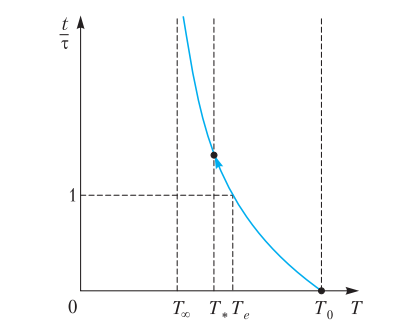
\includegraphics[width=0.4\textwidth]{pic1.png}
    	\caption{Со временем экспоненциально уменьшается температура; $T_e$
    		– значение температуры, достигаемое по истечении характерного
    		времени t = $\tau$ (времени релаксации)}
    \end{figure}

    Что же получается: температура T, входящая в показатель экспоненты (1), сама экспоненциально зависит от времени! Подставив (\ref{myeq:one}) в (1), найдем выражение для скорости экстракции кофе, пропорциональное функции
    \begin{myequation}\label{myeq:two}
    	exp\left[-\frac{Q}{kT_0}\frac{1+a}{1+a exp(-\frac{t}{\tau})}\right].
    \end{myequation}
	\noindent
    где a = $\frac{T_0 - T_\infty}{T_\infty} = \frac{\delta T_0}{T_\infty}$ - начальный перегрев,
    отнесенный к температуре в окружающем пространстве.
    
    Более того, если заваривать кофе "при нормальных условиях" (как говорят настоящие физики) - температуре 
    0\degree C и давлении в одну атмосферу, то отношение $a = \frac{\delta T_0}{T_\infty} = \frac{100 K}{273,15 K} \approx
    \frac{1}{e}$ и выражение ((\ref{myeq:two})) можно назвать трижды экспоненциальным:
    \begin{myequation}\label{myeq:three}
    	exp\left[-\frac{Q}{kT_0}\frac{exp1+a}{exp1+exp(-t/\tau)}\right],
    \end{myequation}
	а число e = exp1 - Фундаментальной Кофейной Постоянной. До чего же вездесуще основание натуральных логарифмов!\columnbreak
	
	На рисунке 3 представлена качественная зависимость (\ref{myeq:three}) скорости экстракции кофе от времени - следствие подстановки
	данных рисунка 2 в рисунок 1. Результат экстрации
	\setlength{\belowcaptionskip}{-10pt} 
	\begin{figure}[H]
		\centering
		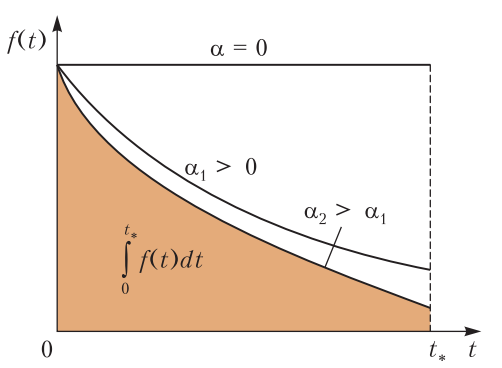
\includegraphics[width=0.4\textwidth]{pic2.png}
		\caption{Зависимость от времени скорости экстракции, учитывающая и ее падение с уменьшающейся температурой (см. рис. 1), и падение
			самой температуры со временем (см. рис. 2);
			D – коэффициент теплообмена с окружающей
			средой. Интеграл по времени от t = 0 до
			заданного t = $t_*$
			– количество экстрагированного вещества}
	\end{figure}
	\noindent
	- это интеграл за все отведенное для заварки время $t_*$, т.е. закрашенная площадь под кривой. Конечно, этот
	результат наиболее впечатляет, если $\alpha = 0$ (нет теплоотдачи в окружающее пространство). Не случайно
	джезву с кофе ставят на раскаленный песок и даже некоторое время кипятят содержимое (<<варят>>).
	
	Вероятно, вдумчивый читатель уже понял, что не следует оставлять ложку в заварной чашке, класть на горку
	молотого кофе лепешку меда или сыпать сахар, которые «оттягивают» на себя часть теплоты кипятка, увеличивая
	теплоотдачу ($\alpha_2 > \alpha_1$), и что сливки нужно добавлять (если, конечно, нужно) при
	$t\geq t_*$, а не раньше. Может быть, этого не знала одна из героинь А.П. Чехова, которая <<...кофий сегодня пила,
	и без всякого удовольствия>>. Но Вы-то всё поняли?
	
	Приятного аппетита!
\end{multicols}
\newpage
\begin{multicols}{2}
	\begin{figure}[H]
		
\includegraphics[width=0.4\textwidth]{pic4}
		\centering
	\end{figure}
Заключительный этап Всероссийской математической олимпиады школьников прошел в
Пермском крае с 21 по 27 апреля 2019 года. Все
участники олимпиады проживали в корпусах
расположенного на живописном берегу Камы
курорта Усть-Качка, а туры олимпиады проходили в находящемся неподалеку современном
здании Кадетского корпуса. В экскурсионную
программу олимпиады были включены поездки в Кунгурскую пещеру, осмотр достопримечательностей Перми. Интересной и насыщенной была научно-познавательная программа
олимпиады: перед участниками выступали с
лекциями представители ведущих университетов страны.

В олимпиаде приняли участие 378 юных
математиков из 65 регионов России. Кроме
того, традиционными участниками олимпиады
\vspace{-2em}
\begin{table}[H]
	\centering
	\caption{9 класс}
	\begin{tabular}{|M{17mm}|M{4mm}|M{4mm}|M{4mm}|M{4mm}|M{4mm}|M{4mm}|M{4mm}|M{4mm}|}
		\hline
		Номер задачи & 1 & 2 & 3 & 4 & 5 & 6 & 7 & 8 \\	
		\hline
		Количество участников (из 130), решивших задачу & 114
		& 38 & 66 & 3 & 93 & 101 & 30 & 3 \\
		\hline
	\end{tabular}
\end{table}
\vspace{-2em}
\begin{table}[H]
	\centering
	\caption{10 класс}
	\begin{tabular}{|M{17mm}|M{4mm}|M{4mm}|M{4mm}|M{4mm}|M{4mm}|M{4mm}|M{4mm}|M{4mm}|}
		\hline
		Номер задачи & 1 & 2 & 3 & 4 & 5 & 6 & 7 & 8 \\	
		\hline
		Количество участников (из 119), решивших задачу & 115
		& 102 & 46 & 13 & 92 & 90 & 85 & 2 \\
		\hline
	\end{tabular}
\end{table}
\vspace{-2em}
\begin{table}[H]
	\centering
	\caption{11 класс}
	\begin{tabular}{|M{17mm}|M{4mm}|M{4mm}|M{4mm}|M{4mm}|M{4mm}|M{4mm}|M{4mm}|M{4mm}|}
		\hline
		Номер задачи & 1 & 2 & 3 & 4 & 5 & 6 & 7 & 8 \\	
		\hline
		Количество участников (из 129), решивших задачу & 126
		& 84 & 36 & 7 & 111 & 91 & 7 & 2 \\
		\hline
	\end{tabular}
\end{table}

\end{multicols}
